\begin{filecontents*}{\jobname.xmpdata}
	\Title{Windows GUI}
	\Author{Markus Himmel}
	\Keywords{operating systems\sep Windows\sep graphical user interfaces}
\end{filecontents*}

\RequirePackage[l2tabu,orthodox]{nag}
\documentclass[10pt,twocolumn,a4paper]{article}
\usepackage[a-1b]{pdfx}
\usepackage[utf8]{inputenc}
\usepackage[T1]{fontenc}
\usepackage[english]{babel}
\usepackage{lmodern}
\usepackage{microtype}
\usepackage{amsmath}
\usepackage{amssymb}
\usepackage{mathtools}
\usepackage{csquotes}
\usepackage{graphicx}
\usepackage{tikz}

\usepackage[margin=1.88cm]{geometry}

\usepackage[
	backend=biber,
	citestyle=numeric-comp
]{biblatex}
\addbibresource{gui.bib}

\usepackage[os=win]{menukeys}

\hypersetup{hidelinks,pdfencoding=unicode}
\usepackage[all]{hypcap}

\author{Markus Himmel}
\title{Windows GUI}

\newcommand{\bs}[1]{\textbf{\sffamily #1}}
\newcommand{\winver}[1]{$^{\text{\hyperref[tbl:abbrev]{\bs{#1}}}}$}
\newcommand{\winsection}[2]{\section{#1\winver{#2}}[#1]}
\newcommand{\winsubsection}[2]{\subsection[#1]{#1\winver{#2}}}

\begin{document}
	\maketitle

	\begin{abstract}
		The graphical user interface is one of the most important components
		of a consumer-oriented operating system such as Microsoft Windows. As
		such, its proper functioning is crucial to the operating system's success.

		This report examines the components of the Windows operating system
		that contribute to the graphical user interface, both from an
		application programmer's and a system architect's point of view. The
		APIs presented to application programmers to register GUI applications
		and to draw graphical applications to the screen are reviewed. In addition,
		implementation details of the graphical user interface and window management
		are examined.
	\end{abstract}

	\section{Introduction}
		A \textit{graphical user interface} (GUI) is a means of communicating
		with an electronic device such as a personal computer that uses graphical
		icons and other visual elements to represent application state. In
		contrast, classical command-line interfaces represent program state to
		the user using text-based representations. In addition, when a GUI is
		in use, the user is able to manipulate application elements using graphical
		means, for example by selecting or dragging with a computer mouse.

		An important reason for choosing a graphical user interface for an
		application over a text-based one is that in some cases, graphical
		representations of application state give access to more intuitive and
		better metaphors, i.e., appropriate images and icons better represent
		the real-world situtations a computer program models and the ways they
		interact than a text-based interface could.

		For these reasons, consumer-oriented desktop operating systems have
		shipped with graphical user interfaces for more than two decades. While
		there is a small degree of
		compatibility and interoperability, all major operating systems such
		as Microsoft Windows, the Mac OS line of operating systems as well
		as the various desktop environments available for GNU/Linux
		provide their own implementation of a graphical user interface. This
		report aims to present an overview over the implementation of the
		graphical user interface of Microsoft Windows.

		Rigorously defining requirements for an efficient graphical user
		interface is outside the scope of this report. Instead, we will focus
		on one particular aspect: Responsiveness. Users perceive the response
		of a computer as \enquote{instantaneous} if the response time is less
		than 100 milliseconds \cite{miller1968response}. Ensuring that as
		little of that time as possible is used for drawing the application on
		the screen is key to the usability of a graphical user interface.

		This report is structured into two parts. Sections~\ref{sec:win32gui} and
		\ref{sec:win32drawing} describe the Windows GUI from an application
		programmer's point of view: Section~\ref{sec:win32gui} describes common
		elements of all Win32 GUI applications and Section~\ref{sec:win32drawing}
		gives an overview over the drawing APIs available to Windows GUI developers.
		The remainder of the report explores the infrastructure enabling
		these features---Section~\ref{sec:win32k} describes the central kernel component
		for the Windows GUI and Section~\ref{sec:wm} discusses window management.

		\subsection{How to Read This Document}
			The Windows NT operating system has seen 12 major revisions over its
			decades-long lifespan, and many of the features described in this
			report differ from version to version. At the same
			time, documentation of the architecture of the Windows GUI is
			scarce.  For this reason, it is not possible to present a
			consistent exposition of the Windows GUI architecture of
			some fixed Windows version.  Instead, different sections of this
			report may be based on different versions of Windows. In order to
			aid the reader in keeping track of which version of Windows is
			being examined, sections and sometimes
			single paragraphs and sentences will be annotated with the Windows
			versions they describe. Here is an example:

			\vspace{1em}
			GDI is not hardware-accelerated.\winver{V}
			\vspace{1em}

			Table~\ref{tbl:abbrev} lists all abbreviations used in this document
			and the Windows versions they refer to.

			In some cases, no documentation of a particular implementation detail
			may exist for any Windows version. In this situation, the author of
			this report used the source code of the ReactOS project,
			a free operating system that aims for binary compatibility with the
			NT family of operating systems \cite{reactos}, in order to
			at least present \emph{an} implementation, without intending to imply
			that this implementation is similar to that of any real Windows version.

			\begin{table}[h]
				\centering
				\begin{tabular}{r|l}
					Abbreviation & Windows Version \\
					\hline
					\bs{NT4} & Windows NT 4.0 \\
					\bs{V} & Windows Vista (\enquote{Longhorn}) \\
					\bs{7} & Windows 7 \\
					\\
					\bs{ROS} & ReactOS source code
				\end{tabular}
				\caption{Abbreviations for Windows versions used in
					this document}
				\label{tbl:abbrev}
			\end{table}

	\section{Win32 GUI Applications}\label{sec:win32gui}
		This section gives a broad overview over Windows GUI applications from an
		application developer's point of view. It will serve as a starting point
		for the deeper investigation of implementation details in the following
		sections.

		\subsection{Window Classes and Objects}
			The fundamental building block of a Windows GUI application is the
			\textit{window object}, typically just referred to as \textit{window} \cite{whatiswindow}.
			Window objects are not only windows in the colloquial sense, but also
			most types of controls found inside application windows, such as buttons
			or text boxes. Windows are organized in a hierarchical structure.
			Top-level windows do not have a parent window and are referred to as
			\textit{application windows}. Every window has zero or more child
			windows. Application windows consist of two parts: The \textit{non-client
			area} consists of the frame of the window, including the title bar and
			controls like the close button. It is drawn by the operating system.
			The \textit{client area} is the part of the window that is drawn by
			the application itself
			\cite{whatiswindow}.

			Each window object is an instance of a given \textit{window class} \cite{creatingwindow}.
			Window classes, while conceptually comparable, are not classes in
			the object-oriented programming sense. Instead, windows classes are
			registered with the kernel at runtime and can then be instantiated.
			Window classes determine the appearance and behavior of a window.
			Application developers create instances of a window class
			using the function
			\texttt{CreateWindowEx}, which requires the name of the window class
			to instantiate and returns a handle to the newly created window.
			The type of the handle is \texttt{HWND} \cite{whatiswindow}. This type is opaque to the
			application developer. Functions that in some way operate on a
			window object take the \texttt{HWND} as a parameter.

		\subsection{Window Messages and Procedures}
			Window classes determine the behavior of window objects \cite{creatingwindow}. The mechanism
			through which window object behavior is defined is the reaction of
			a window object to messages sent to the object. The callback that
			the application calls when it receives a window message
			for a window object from the kernel is called
			\textit{window procedure} \cite{aboutwinproc} and is part of the window class, i.e., when
			registering a window class, application developers must provide a
			pointer to the window procedure for the window class. The window
			procedure requires four parameters: The \texttt{HWND} of the window
			object that received the window message, a numeric code detailing the
			type of the message received, and two parameters for the message
			\cite{aboutwinproc}.

			A window procedure handles some of the messages it receives.
			Typical types of messages are requests to repaint some region of
			the window, notifications about user input, or the notification
			that the application is about to exit. If a message is not handled
			by the window procedure, the window procedure must call
			\texttt{DefWindowProc}, resulting in execution of a default window
			procedure to ensure that all messages are handled
			\cite{aboutwinproc}. If the window procedure does not call the
			default procedure, it has to implement the functionality of the
			default window procedure itself in order for the graphical user
			interface to work. For example, when the application calls
			\texttt{CreateWindow},
			the window procedure receives a \texttt{WM\_NCCREATE}
			message \cite{createwindow}. This message expects the window procedure
			to return a non-zero value if creation of the window should continue
			\cite{wmnccreate},
			so if the default window procedure is not called the window procedure
			must specifically handle this message, otherwise \texttt{CreateWindow}
			returns a \texttt{NULL} \texttt{HWND}.

			In order to support this message-driven mode of operation, the main
			thread of every Windows GUI application is required to execute a
			message loop immediately after creating the main application
			window\footnote{In particular, creation of components on the main
			window is performed in the message handler for the
			\texttt{WM\_CREATE} message \cite{usingwindows}, so the main application window does
			not display any controls or content before the main thread enters
			the message loop.} \cite{messages}. Applications may fetch the next message in the
			queue using \texttt{GetMessage}. The application then has to pass
			the message first to \texttt{TranslateMessage} and then to
			\texttt{DispatchMessage} \cite{usingwindows}. \texttt{TranslateMessage} translates key
			code messages returned by the keyboard driver into Unicode
			characters according to the current keyboard layout and posts new
			messages with these characters to the application \cite{translatemessage}. This is a step performed
			by the application itself instead of the operating system because
			there are some cases where an application wants to process the virtual
			key codes instead of the mapped ones \cite{translatemessage} and because the current keyboard
			layout depends on the current thread, so the kernel thread generating
			the messages is by itself unable to map virtual key codes to actual
			key codes\winver{ROS}. \texttt{DispatchMessage} then invokes the window procedure
			of the window object the message was posted to \cite{dispatchmessage}. The target \texttt{HWND}
			is part of the message record fetched by \texttt{GetMessage} \cite{msgstruct}.


	\section{Win32 Drawing APIs}\label{sec:win32drawing}
		\begin{figure*}
			\centering
			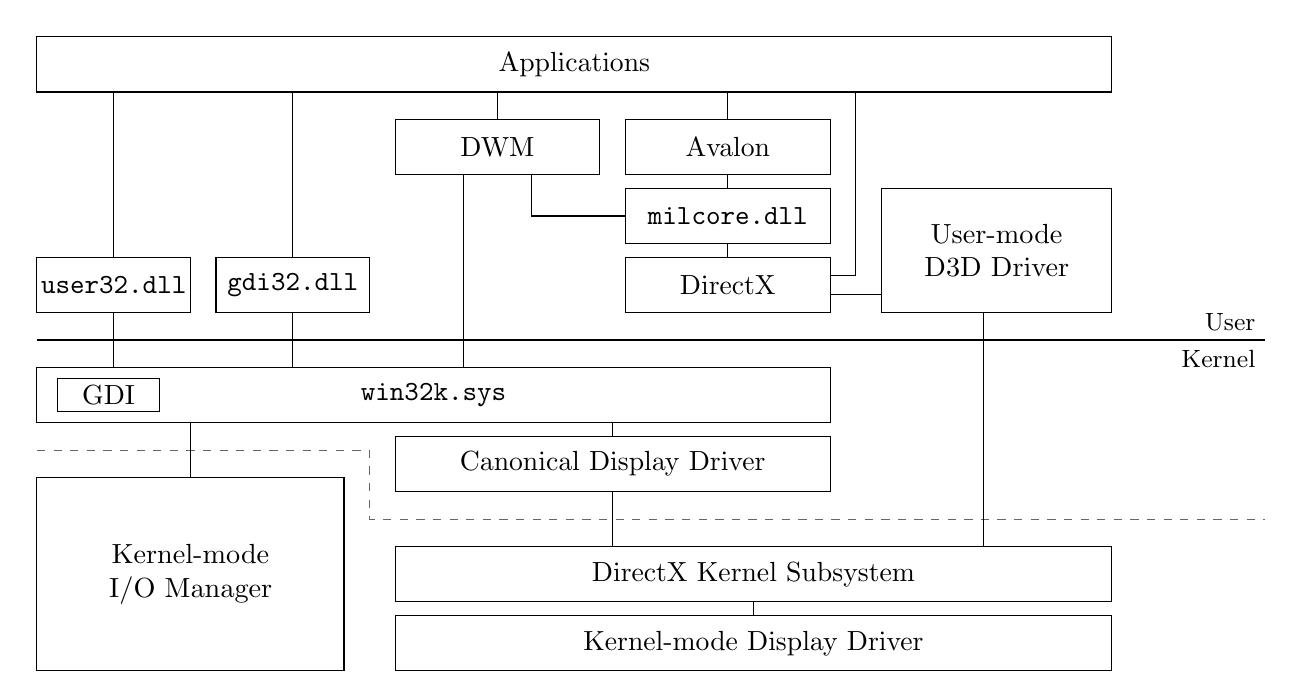
\begin{tikzpicture}[yscale=0.7, xscale=1.3]
				\node at (0, 0) {};
				\node at (12, 10.5) {};
				\draw[thick] (0, 5) -- (12, 5);
				\node[anchor=south east] at (12, 5) { \small User };
				\node[anchor=north east] at (12, 5) { \small Kernel };
				\draw (0, 9.5) rectangle node (apps) { Applications } ++(10.5, 1);
				\draw (0, 5.5) rectangle node { \texttt{user32.dll} } ++(1.5, 1);
				\draw (0.75, 6.5) -- ++(0, 3);
				\draw (0, 3.5) rectangle node { \texttt{win32k.sys} } ++(7.75, 1);
				\draw (0.75, 4.5) -- ++(0, 1);
				\draw (0, -1) rectangle node[align=center,text width=2.5cm] { Kernel-mode I/O Manager } ++(3, 3.5);
				\draw[dashed,color=black!60] (0, 3) -- (3.25, 3) -- (3.25, 1.75) --
					(12, 1.75);
				\draw (1.5, 2.5) -- ++(0, 1);
				\draw (1.75, 5.5) rectangle node (gdi32) { \texttt{gdi32.dll} } ++(1.5, 1);
				\draw (2.5, 6.5) -- ++(0, 3);
				\draw (2.5, 4.5) -- ++(0, 1);
				\draw (0.2, 3.7) rectangle node { GDI } ++(1, 0.6);
				\draw (3.5, -1) rectangle node { Kernel-mode Display Driver } ++(7, 1);
				\draw (3.5, 2.25) rectangle node { Canonical Display Driver } ++(4.25, 1);
				\draw (3.5, 0.25) rectangle node { DirectX Kernel Subsystem } ++(7, 1);
				\draw (7, 0) -- ++(0, 0.25);
				\draw (9.25, 1.25) -- ++(0, 4.25);
				\draw (5.625, 3.25) -- ++(0, 0.25);
				\draw (5.625, 1.25) -- ++(0, 1);
				\draw (5.75, 5.5) rectangle node { DirectX } ++(2, 1);
				\draw (5.75, 6.75) rectangle node { \texttt{milcore.dll} } ++(2, 1);
				\draw (8.25, 5.5) rectangle node[align=center,text width=2.5cm] { User-mode D3D Driver } ++(2.25, 2.25);
				\draw (5.75, 8) rectangle node { Avalon } ++(2, 1);
				\draw (7.75, 5.5+2/3) -| ++(0.25, 3+1/3);
				\draw (6.75, 9) -- ++(0, 0.5);
				\draw (6.75, 7.75) -- ++(0, 0.25);
				\draw (6.75, 6.5) -- ++(0, 0.25);
				\draw (7.75, 5.5+1/3) -- ++(0.5, 0);
				\draw (3.5, 8) rectangle node { DWM } ++(2, 1);
				\draw (4.5, 9) -- ++(0, 0.5);
				\draw (5.75, 7.25) -| ++(-0.25-2/3, 0.75);
				\draw (3.5+2/3, 8) -- ++(0, -3.5);
			\end{tikzpicture}
			\caption{An overview of the Windows GUI architecture, showing both user-mode
				and kernel-mode components involved in rendering the Windows GUI. The
				diagram assumes a machine running Windows Vista using a Vista-ready
				GPU with appropriate drivers.}
			\label{fig:arch}
		\end{figure*}
		After registering a window, an application has to draw its client area
		to the screen. Windows provides multiple APIs to accomplish this task.

		\winsubsection{Graphics Device Interface}{V} \label{sec:gdi}
			\textit{Graphics Device Interface} (GDI) is the oldest drawing API
			that is available in modern Windows versions. Unlike the other
			APIs presented in this report,
			it predates modern 3D acceleration units and as such
			was not designed for GPU hardware acceleration. Instead, it was
			designed to operate using the CPU and supports its own driver model
			for hardware acceleration called \textit{GDI Device Driver
			Interface} (DDI) specifically for accelerating GDI
			primitives \cite{d2dvsgdi}. When the DDI was created, hardware that is able to
			accelerate the specific operations used in GDI existed, but modern GPUs operate
			very differently and cannot provide hardware acceleration. As such,
			GDI operations always run on the CPU on Windows Vista \cite{d2dvsgdi}.

			GDI functions are provided by the user space module
			\texttt{gdi32.dll} which in turn calls into the GDI kernel residing
			in \texttt{win32k.sys} \cite{d2dvsgdi}. The GDI kernel communicates with the
			system's DDI driver. Windows Vista only supports a single DDI driver,
			the \textit{Canonical Display Driver} \cite{d2dvsgdi}, which renders requested operations
			into a buffer located in main memory \cite{dwmredirect}. Refer to Figure~\ref{fig:arch}
			for an overview.

		\subsection{DirectX}
			Microsoft \textit{DirectX} is a collection of APIs exposing functionality of
			a GPU to application developers. While originally intended for
			multimedia applications such as video playback and video games, it
			is now also used for regular GUI applications and multiple specific
			APIs have been added to the collection over the years to further
			facilitate this use case, with the intention to ultimately replace GDI, at
			least for new applications \cite{aboutd2d}.
			Unlike GDI applications, DirectX applications
			are rendered by the GPU into video memory \cite{d2dvsgdi}.

			In the context of graphics programming, the most fundamental part of
			DirectX is Direct3D, which provides support for 3D graphics. The
			APIs tailored towards traditional GUI developers, Direct2D and
			DirectWrite, are implemented on top of Direct3D \cite{aboutd2d}.

		\winsubsection{Avalon}{V}\label{sec:milcore}
			Unlike GDI and DirectX, \textit{Avalon}, also known as \textit{Windows Presentation
			Foundation} (WPF),
			is not a low level drawing framework
			that communicates directly with a graphics driver, but a
			high level GUI framework available to CLR\footnote{The \textit{Common
			Language Runtime} (CLR) is a runtime system comparable to the Java Virtual
			Machine. It runs \textit{Common Intermediate Language} (CIL) bytecode.
			The most well-known programming language targeting the CLR is Microsoft
			C\#.} applications \cite{goingdeep}. Avalon is
			implemented on top of DirectX \cite{dwmwpf}. The major rendering work is performed
			by a native module called \texttt{milcore.dll} (where MIL is short for
			\textit{Media Integration Layer}). Avalon applications maintain a
			so-called \textit{visual tree} on their UI thread\footnote{An
			earlier implementation using a rental threaded model where every
			application thread was allowed to modify UI elements was scrapped
			for interoperability reasons \cite{goingdeep}.} which represents the
			client area of the application. An unmanaged portion of the UI thread
			code then communicates the visual tree to a \texttt{milcore}-provided
			rendering thread which keeps its own copy of the tree \cite{goingdeep}. In some situations,
			raw image data is shared between the UI thread and the rendering thread. The
			rendering thread then walks the visual tree and issues the correct
			DirectX commands to draw the application \cite{goingdeep}.

			Decoupling the UI thread from the rendering thread comes with
			advantages. Not having to wait for rendering to finish before being
			able to make changes to the UI can improve application performance.
			Conversely, being able to render despite a busy UI thread improves
			application responsiveness as perceived by the user. Additionally,
			separating the two tasks allows for \textit{remoting}, i.e., running
			an application and its UI thread on a server and displaying it
			via a rendering thread running on a client. Since both client and
			server maintain the visual tree, updates in the user interface can
			efficiently be communicated to the client using deltas to the visual
			tree \cite{goingdeep}.

			When the rendering thread is notified of a change to the visual tree,
			it updates the application on the screen. This step is performed by
			traversing the visual tree and drawing each component of the tree.
			However, if rendering occurs in response to a change to the visual
			tree, not the entire visual tree is redrawn \cite{goingdeep}. Instead, \texttt{milcore}
			employs dirty region management and occlusion culling---i.e.,
			determining which elements of the tree are visible at a particular
			moment. These optimizations ensure that no unnecessary rendering takes
			place \cite{goingdeep}.

		\subsection{Cross-platform Graphics APIs}
			Beside the essentially Windows-specific DirectX API, there are
			several cross-platform APIs that aim to fill a similar
			niche\footnote{Notably, DirectX does not fill a single niche. In
			particular, different versions of the DirectX API emphasize
			different usage models.  DirectX version 11 and before are most
			comparable to OpenGL in being relatively high-level. In contrast,
			DirectX 12 is more low-level and thus similar to Vulkan.}.
			Targeting cross-platform APIs instead of DirectX enables running
			software on different platforms and operating systems with minimal
			adjustments, which makes the application available to a larger
			audience. Of these, two are available on Windows: OpenGL and
			Vulkan, an API for low-level access to graphics hardware
			\cite[3]{vulkanspec}. Since, unlike DirectX, these APIs are not as
			tightly integrated
			into the Windows operating system, the most interesting question is
			how the interface between the Win32 API and the cross platform API
			is implemented, i.e., how the application programmer can obtain an
			API-specific surface for the client area of an \texttt{HWND}.

			OpenGL is officially supported by Windows. Drivers for OpenGL are
			loaded through a mechanism called \textit{installable client
			drivers} (ICDs) \cite{oglicd}. Microsoft provides a module called
			\texttt{opengl32.dll} which checks a specific registry key
			for a vendor-provided OpenGL driver. If such a driver is found,
			OpenGL calls are relayed to this driver. Otherwise, a
			default implementation provided by Microsoft is used \cite{oglcomp}. Regardless
			of which OpenGL implementation is used, Windows OpenGL applications
			first obtain a GDI device context via the standard GDI function
			\texttt{getDC(HWND)} and then pass this device context to the
			Microsoft-provided function \texttt{wglCreateContext} to obtain an
			OpenGL rendering context for use in the cross-platform portion
			of the application \cite{oglrc}.

			Support for graphics software that uses the Vulkan API is not
			directly built into Windows as in the OpenGL case. Instead,
			Khronos, the working group that authored the Vulkan specification,
			provides a loader that searches for Vulkan-compatible display
			drivers using an installable client driver model similar to that of
			OpenGL \cite{vulkanloader}. Vulkan specifies a Windows-specific
			extension to create a Vulkan surface that corresponds to the client
			area of an \texttt{HWND}: \texttt{vkCreateWin32SurfaceKHR}. Once
			this surface has been created, the rest of the code of a Vulkan
			application is platform-agnostic \cite[799]{vulkanspec}.

	\section{NT Kernel Support for GUI Applications}\label{sec:win32k}
		The functions available to the user for creating GUI applications are
		exported by \texttt{user32.dll}, which is a user-space library.
		However, the actual functionality is provided by a kernel module called
		\texttt{win32k.sys} \cite{probertwin32k}. Refer to Figure~\ref{fig:arch} for an overview over the
		components involved in the Windows graphical user interface.

		\texttt{win32k} maintains a list of all active GUI threads of the
		current session. A GUI thread is somewhat circularly defined as a
		thread that is known to \texttt{win32k} as a GUI thread \cite{probertwin32k}. Upon creation,
		a thread is not a GUI thread. A thread is promoted to a GUI thread when
		it first calls into \texttt{win32k}, for example when calling
		\texttt{CreateWindowEx} from \texttt{user32.dll}. After a thread is
		promoted, \texttt{win32k} becomes aware of the thread (and in
		particular, is notified of its destruction \cite{probertwin32k}). In addition, the thread
		receives a bigger kernel stack, because \texttt{win32k} call chains
		can become rather deep and some specific mechanisms employed by \texttt{win32k}
		require extra stack space \cite{mandy2011kernel}.

		Besides managing GUI threads, \texttt{win32k} contains the kernel portion
		of window management \cite{probertwin32k}. It responds to requests to create and close windows
		and keeps a list of all top-level windows of the window station \cite{goingdeep}.

		Another major responsibility of \texttt{win32k} is the \textit{raw input
		thread} (RIT). The raw input thread is responsible for receiving user input and posting
		messages to the correct window\footnote{Implementation details of the
		RIT appear to be undocumented. The ReactOS implementation of
		the Raw Input Thread continuously and actively polls mouse and keyboard
		in turn. If the driver returns a new input, the recipient top-level \texttt{HWND}
		is determined. In case of keyboard input or a mouse event while the mouse
		has been captured by an application, the active or capturing application
		receives the message, respectively. In case of a mouse event while the
		mouse is not caputured, all top-level windows are enumerated and the
		window the mouse is above is selected.\winver{ROS}} \cite{probertwin32k}.

		\winsubsection{Moving \texttt{win32k} to the Kernel}{NT4}
			It is possible to provide the functionality described in
			Section~\ref{sec:win32k} using a user-space module. Even further,
			proper microkernel design principles mandate that \texttt{win32k}
			\emph{must} be placed in user space, because it is not inherently
			reliant on kernel-mode functionality.  In fact, Windows versions
			prior to Windows NT 4.0 do implement \texttt{win32k} functionality
			in user space by having applications communicate with the
			user-space \textit{Client-Server Subsystem} (CSRSS) which contains
			\texttt{win32k} and communicates with the kernel for low-level
			operations such as calls to the graphics hardware. Note the
			additional layer of indirection compared to other operating system
			interfaces, where applications make system calls directly
			\cite{gdikernel}.

			In Windows NT 4.0 \texttt{win32k} was moved to kernel space for
			performance reasons \cite{gdikernel}. Performance problems with the
			CSRSS approach stem from both the fact that inter-process
			communication has to be employed by applications in order to
			communicate with CSRSS and the need for memory to be shared across
			the kernel mode boundary for CSRSS to provide its functionality
			\cite{gdikernel}. On a typical machine running Windows NT 4.0, a
			kernel-mode transition was measured to take four to five
			milliseconds, compared to 60 to 70 milliseconds for an
			inter-process call to CSRSS \cite{gdikernel}.

			Windows NT 3.51 contains a large number of optimizations to be able
			to support a user-space \texttt{win32k}, many of them related to
			efficient execution of GDI operations (see Section~\ref{sec:gdi}).
			For example, GDI operations requested by the application are not
			actually drawn immediately by calling into CSRSS. Instead, GDI
			operations are placed in a queue. Once the queue is full or is
			flushed manually by the application, \texttt{gdi32} communicates
			with CSRSS and executes all queued operations in sequence.
			Symmetrically, \texttt{win32k} data which is available to the
			application is cached by the application \cite{gdikernel}.

			Moving \texttt{win32k} to the kernel eliminates the indirection of
			the client/server approach, which saves both processor time lost
			performing client/server transitions and the overhead associated
			with sharing memory. In order to limit the amount of required
			kernel-mode transitions, a limited degree of batching is still
			performed \cite{gdikernel}.

			The architectural justification for this change is that the
			subsystem retains its microkernel-like interface while providing
			significantly improved performance. This style of kernel
			architecture is referred to as \emph{modified microkernel}
			\cite{gdikernel}.

			Moving \texttt{win32k} from user mode to kernel mode without
			fundamentally adapting its architecture---which would be very
			challenging due to compatibility---has created an entire class of
			security problems \cite{mandy2011kernel}.  In several situations arising in the context of
			\texttt{win32k}, calling back from the kernel into user-mode code
			(rather than just returning) is necessary. In order to facilitate
			this, \texttt{win32k} provides a mechanism called \textit{user-mode
			callbacks}. This functionality has shown to be very prone to
			creating security problems, such as information leakage or
			transitioning back into user mode after a different code execution
			vulnerability has already been exploited \cite{mandy2011kernel}.

	\section{Window Management}\label{sec:wm}
			The window manager is the component of a window-based graphical user
			interface that is responsible for managing the position of each active
			window on the desktop and making sure the desktop as the sum of its
			parts is assembled correctly. There are two general approaches to this
			task: \emph{non-compositing} and \emph{compositing} window management.

			A non-compositing window manager draws non-window elements of the
			desktop (such as the taskbar or equivalent) and maintains the
			position and relative order of all currently visible windows. It
			then instructs applications to draw the currently visible portion
			of their windows directly onto the screen buffer. In particular,
			this means that all applications draw to the same memory buffer and
			when a window is moved on top of another window, that window's data
			is overwritten.

			Non-compositing window managers are efficient and
			straightforward to implement. However, there are drawbacks
			to this approach. It inherently comes
			with visual artifacts. Because window contents are drawn
			directly on the screen without any form of double buffering, screen
			tearing is visible during high-motion events such as scrolling
			text. Additionally, in a situation where a window is moved on top
			of an unresponsive window and subsequently moved away, requests to
			redraw the region of the bottom window which is now visible again
			are sent, but not handled because the application is not
			responsive. The result is the well-known \enquote{trail} effect
			observed in old versions of Microsoft Windows. Refer to
			Figure~\ref{fig:trail} for an example of the problem.
			\begin{figure}[h]
				\centering
				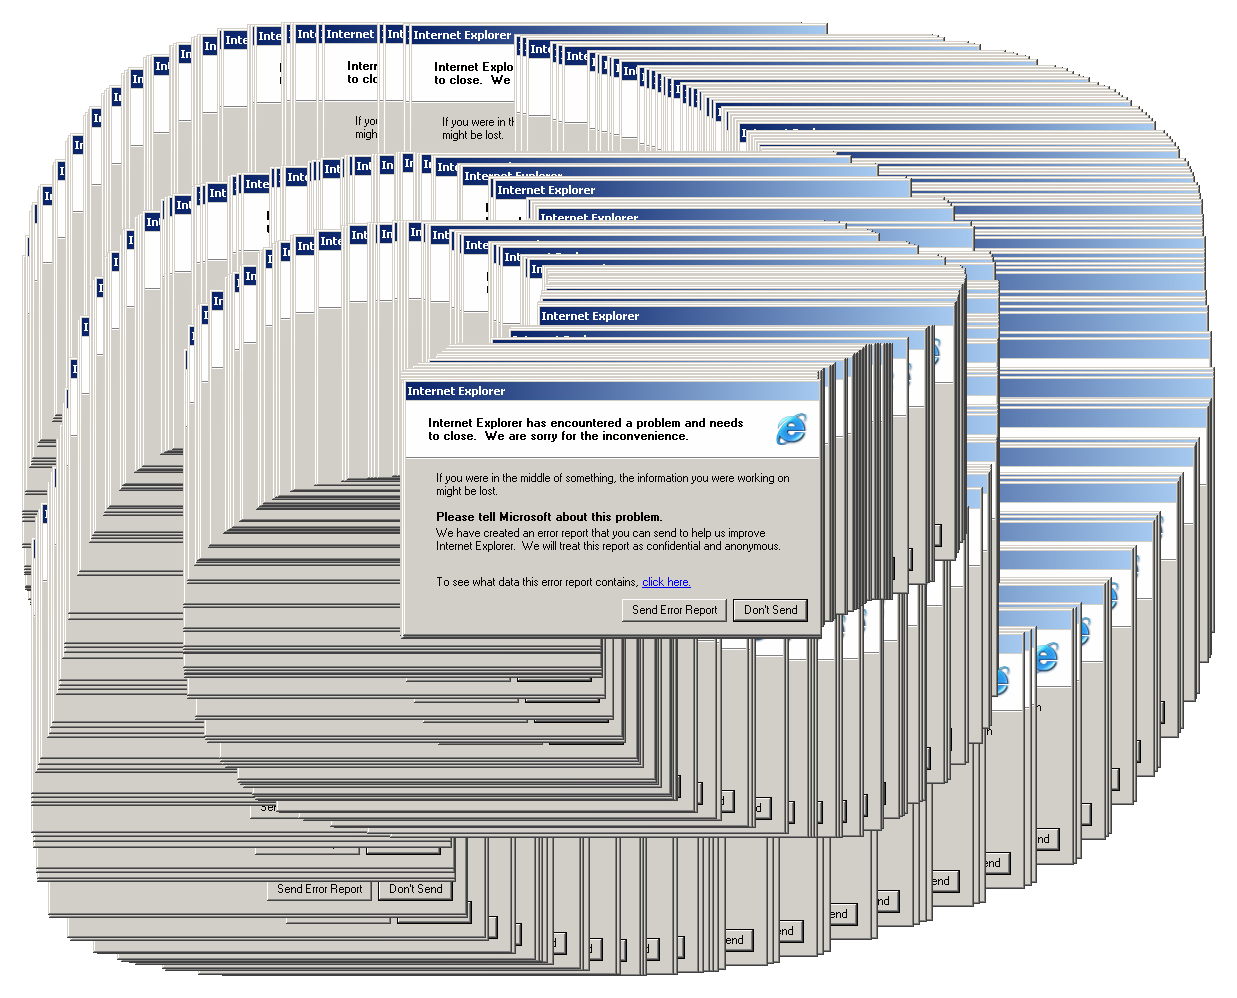
\includegraphics[width=0.8\columnwidth]{trail}
				\caption{The \enquote{trail} effect observed on pre-Vista versions
					of Windows. An application is moved on top of another application
					and then moved away. When the top window is moved away, the bottom
					application needs to redraw the uncovered region. If it does not
					respond to the repaint message, the moved portions of the top
					window are not erased.}
				\label{fig:trail}
			\end{figure}

			Another shortcoming of non-compositing window managers is their
			inability to provide visual effects. As a consequence of the fact
			that (at most) one application determines the color of each individual
			pixel on the screen, effects such as partially transparent windows
			cannot be realized with non-compositing window managers. Additionally,
			because a window may only be at most at one position of the screen,
			and that position has to be the window's \enquote{actual} position,
			no thumbnails or overviews of windows can be shown.

			Compositing is an attempt at a solution to the aforementioned
			problems.  If a compositing window manager is in use, applications
			do not draw directly to the screen. Instead, each application has
			its own off-screen buffer. The
			window manager then assembles the final
			desktop from the content of these buffers. It is immediately clear how this approach addresses the
			problems of non-compositing window-managers described above: It is
			easy to perform double buffering and even when a window is not
			responding, the window manager knows its last good state and can
			use it to prevent trails. Furthermore, visual effects are trivial
			to achieve when compositing is used \cite{dwmoverview}.

		\winsubsection{The Desktop Window Manager}{V}\label{sec:dwm}
			The \emph{Desktop Window Manager} (DWM) is the compositing window
			manager used by Windows and introduced in Longhorn
			\cite{dwmoverview}. It is implemented as a full-screen Direct3D
			user-space application \cite{dwmdirectx}. In particular, DWM rendering is
			hardware-accelerated. When DWM is active, applications render into
			off-screen DirectX buffers which are mapped onto flat surfaces in
			3D space and rendered by the graphics hardware. This design supports
			applying three-dimensional transformations to windows,
			which is used for the
			\enquote{Flip3D} feature of Windows Vista invoked by the keyboard
			shortcut \keys{Win+\tab} and similar features included in more
			recent versions of Microsoft Windows. Visual effects such as
			transparency are implemented using DirectX pixel shaders. In addition,
			double buffering is implemented using a buffer flipping mechanism
			native to DirectX \cite{dwmdirectx}.

			Even though DWM is a native application, its implementation closely
			resembles that of an Avalon application \cite{dwmwpf}. In particular, the desktop
			is modeled as a visual tree in the same way that WPF applications
			are modeled as a visual tree (refer to Section~\ref{sec:milcore}
			for details) and DWM also uses \texttt{milcore.dll} to render the
			visual tree through DirectX \cite{goingdeep}. This code reuse provides a
			substantial number of necessary functional and performance
			features essentially for free \cite{dwmwpf}.  In particular, the visual tree
			model, which at first might appear not to fit a mostly
			non-hierarchical situation such as the desktop very well,
			turns out to be very beneficial, since the Avalon composition
			engine comes with support for occlusion culling---i.e.,
			determining which parts of a window are visible at a particular
			moment. This feature completely takes care of the task to
			determine which parts of a window should be redrawn. Similarly, the
			entire logic that decides when to request which region of which window
			to redraw (scheduling and dirty region management) is identical to
			its counterpart in Avalon \cite{dwmwpf}.

			The visual \enquote{tree} as employed by DWM allows for non-tree edges
			in order to render windows at locations different from their \enquote{actual}
			position \cite{goingdeep}. This feature is used to implement thumbnails and previews.
			Another use of this feature is the \enquote{magnifier} accessibility
			feature, which renders a portion of a screen in a larger region.
			It is implemented by additionally applying a transform to the entire
			subtree that the virtual edge points to in order to render into a
			magnified buffer\footnote{In addition, special care is taken by the
			application
			that this virtual edge is not traversed once again, which would result
			in an unwanted instance of the Droste effect, i.e., the scaled region
			of the screen recursively appearing within itself
			\cite{goingdeep}.} \cite{goingdeep}.
			For most applications, this means that the pixels are scaled up naïvely.
			However, Avalon applications come with special support for magnification,
			resulting in a pixel-perfect magnified presentation. This support
			is enabled by specific handling in Avalon---in particular, the DWM's
			visual tree does \emph{not} have access to the visual tree of an
			Avalon application \cite{goingdeep}.

			The way in which windows are redirected when DWM is in use depends
			on the drawing API used by the application. GUI applications which
			(directly or indirectly)
			use DirectX for rendering can render into a single buffer located
			in video memory allocated
			by the DWM. Because DWM itself uses DirectX, DirectX applications
			natively render into the format used by DWM, so the DWM can use
			these buffers directly to perform composition
			\cite{dwmredirect}.

			Applications employing GDI for their rendering cannot render into
			the DirectX pixel format, but render into a DWM-provided main memory
			buffer in their native GDI format \cite{goingdeep}. When the window is created, DWM
			automatically also creates a DirectX buffer in video memory. The
			application draws into the GDI buffer, and DWM manually transcribes
			the GDI buffer to the DirectX buffer when necessary and uses the result
			for composition
			\cite{dwmredirect}.

		\winsubsection{The Windows Display Driver Mo\-del}{V}\label{sec:wddm}
			The implementation of DWM described in Section~\ref{sec:dwm}
			fundamentally relies on graphics driver support in order to achieve
			acceptable performance \cite{dwmwddm}.  Prior to Longhorn, DirectX applications
			assumed that they have exclusive access to the GPU. In particular,
			there was no virtual memory and no support for preemption. This is
			unproblematic as long as there is at most one active DirectX application
			and that application has predictable video memory requirements \cite{dwmwddm}.
			However, the Desktop Window Manager \emph{is} a DirectX appliction that
			by design both runs alongside other DirectX applications and whose
			memory consumption is dependent on the number of open windows and therefore
			unpredictable.
			In order to address these problems, display drivers targeting Longhorn
			have to implement the Windows Display Driver Model \cite{dwmalwayson}. This
			display driver framework introduces the cooperative multitasking
			features known from regular applications running on the CPU to the
			GPU \cite{dwmwddm}.

			One of these features is an implementation of preemption called
			WDDM \emph{scheduling} \cite{dwmwddm}. The granularity of preemption depends on
			the version of DirectX that is used and hardware support. When
			using \emph{basic scheduling}, available from DirectX 9 without
			special hardware support, primitives and shaders cannot be interrupted,
			so preemption can only take place in between these basic operations.
			If the hardware supports it and DirectX 10 is in use, \emph{advanced
			scheduling} is available, allowing preemption to take place in the middle
			of primitives or shaders \cite{dwmwddm}.

			The other large feature required for cooperative multitasking is
			virtual memory \cite{dwmwddm}. As GPUs may have several regions of video memory
			specialized for certain tasks, the address space of a GPU may
			be nonlinear. For this reason, the GPU announces some number of
			available segments of video memory to the driver framework \cite{gpuseg}.
			When using the WDDM 1.$x$ model for virtual graphics
			memory, applications work with segment physical addresses. In the event
			that a piece of memory is moved or paged out, addresses in the command
			buffer are patched \cite{wddm2}. This model was updated to using proper virtual
			addresses with WDDM 2.0, introduced in Windows 10 \cite{wddm2}.

			Finally, a third feature that is necessary to implement the redirection
			mechanism for DirectX applications described in Section~\ref{sec:dwm}
			is DirectX surface sharing, which gives an application and the DWM
			access to the same DirectX surface buffer, so that the DWM can use the
			same surface for compositing that is used by the application for
			drawing to \cite{dwmredirect}.

			The desktop window manager cannot run without a WDDM-compliant
			display driver \cite{dwmwddm}. If no such driver is available,
			\texttt{win32k} \cite{probertwin32k} performs one of two actions,
			depending on the version of Windows that is running. Under Windows
			Vista and Windows 7, DWM is disabled\footnote{In Windows Vista and
			7, there are some other ways for DWM to be disabled. Applications
			can disable the DWM manually (for example immediately before
			switching to full-screen mode) \cite{disabledwm}. Furthermore, DWM
			shuts down if an application bypasses compositing and instead draws
			directly to the screen \cite{dwmredirect}.} and the non-compositing
			window manager\footnote{Contrary to the DWM, the non-compositing
			window manager referred to as \textit{USER} resides in
			\texttt{win32k} and thus in kernel space \cite{probertwin32k}.}
			from Windows XP is used. When running Windows 8 or later, the DWM
			runs, but a software-based renderer called \textit{Microsoft Basic
			Display Adapter} serves as a replacement for the display driver
			\cite{dwmalwayson}.

			From a GPU driver developer's point of view, a WDDM driver consists
			of a \textit{user-mode display driver} (also referred to as
			\textit{user-mode Direct3D driver}) and a kernel-mode
			\textit{display miniport driver}, sometimes called \textit{kernel-mode
			display driver} \cite{wddmarch}. Both components are solely concerned with handling
			DirectX operations---calls to all other types of graphics API that
			are available on Windows, notably including OpenGL in case the driver
			vendor chooses not to provide a direct implementation of OpenGL via
			an installable client driver, are either not
			hardware-accelerated or relayed to the appropriate DirectX commands
			\cite{d2dvsgdi}.
			Figure~\ref{fig:arch} visualizes the interaction of a WDDM driver with
			other GUI-related components.

		\winsubsection{GDI Hardware Acceleration}{7}
			During Longhorn development, having GDI directly render to DirectX
			surfaces in video memory was deemed infeasible \cite{dwmredirect}. The problem
			was not that GDI calls
			could not be adapted to work with the DirectX buffer format, but
			GDI renders using the CPU and many GDI operations not only write to
			the buffer, but also need to read from it, and reading from video memory
			using the CPU is a very slow operation \cite{dwmredirect}. However,
			Windows 7 does eliminate the main memory buffer for GDI \cite{win7}. The performance
			issues were resolved by providing explicit hardware acceleration for
			the offending GDI operations in WDDM version 1.1. In particular,
			starting with Windows 7, the
			main memory consumption of the Desktop Window Manager is independent
			of the number of open windows (however, VRAM consumption still scales
			linearly with the number of open windows) \cite{win7}.

	\section{Conclusion}
		Microsoft Windows is an operating system with a diverse audience and
		broad requirements in terms of (backwards) compatibility. The design
		of the NT kernel certainly shows its age, especially the parts of the API
		that have remained largely unchanged since the 16-bit era\footnote{Note however,
		that well-designed operating system APIs did exist even in the 1990s, the
		most prominent example perhaps being the almost entirely C++-based Be API,
		which is implemented by the open source Haiku operating system
		\cite{haikuapi} and which the author of this document considers
		progressive even by today's standards.}. Nonetheless, the components have
		proven to be robust enough to be able to adapt to almost three decades'
		worth of new developments in information technology, which is a remarkable
		achievement.

		This report examined the components involved in the graphical user
		interface of the Windows operating system. While it is still possible
		to write GUI applications in almost entirely the same way as when Windows NT
		was in its infancy, the implementation of these features did change, in
		some cases in fundamental ways. It should be noted that many far-reaching
		and forward-thinking
		changes to the graphical user interface were first released in Windows
		Vista. This evidence suggests the conclusion that while Windows Vista itself
		was a commercial failure, it laid the foundation for the success of later
		versions of the Windows operating system.


	\onecolumn{\printbibliography}
\end{document}
